\section{Le visuel en DirectX11}

\subsection{Le rendu visuel du jeu}
Dans ce projet, l’aspect visuel joue un rôle essentiel pour offrir une représentation claire et fluide du jeu. L’objectif était de créer un rendu simple mais efficace, permettant aux joueurs de suivre l’évolution de la partie sans latence ni ambiguïté. Pour cela, nous avons choisi d’utiliser DirectX 11 en C++, une combinaison qui nous permet d’avoir un contrôle total sur l’affichage tout en optimisant les performances.
Dans les sections suivantes, nous détaillerons le fonctionnement du moteur graphique, la manière dont nous avons modélisé les éléments du jeu, les effets visuels implémentés, ainsi que les optimisations mises en place pour assurer un rendu fluide et réactif.

\subsection{Fonctionnement du moteur graphique}
Le fonctionnement du moteur graphique repose sur une architecture assez technique, mais dans cette section, nous allons volontairement éviter les détails trop complexes pour nous concentrer sur l’idée générale. \\
Le jeu tourne à l’intérieur d’une application principale qui gère la création et le rendu de scènes. Une \textbf{scène} représente un état visuel du jeu à un instant donné, et elle est composée d’un ensemble d’objets que nous appelons des \textbf{Drawables}. La scène principale du jeu, celle qui affiche tout ce qui se passe pendant une partie, est appelée GameScene. \\
Les \textbf{Drawables} sont les briques de base de l’affichage. Chaque Drawable représente un objet du jeu (joueur, mur, grille, etc.). Ils sont répartis en trois grandes familles : SingleMeshDrawable, InstanceMeshDrawable et CompositeDrawable, que nous détaillerons plus tard. De manière générale, un Drawable contient un \textbf{Mesh}, c’est-à-dire une structure composée de points \textbf{(vertices)} et de triangles \textbf{(indices)} qui permet de modéliser des formes simples comme un cube ou un cylindre. \\
Le rôle d’un \textbf{Drawable} est d’être préparé pour le rendu. Cela signifie qu’il doit rassembler toutes les données nécessaires (position, couleur, texture, etc.) et les transmettre efficacement à DirectX. Pour cela, nous utilisons des \textbf{Bindables}, qui agissent comme des \textbf{wrappers} autour des appels nécessaires à l’envoi des buffers. Ces buffers, déjà créés en amont, sont ensuite intégrés dans le \textbf{pipeline} de rendu de DirectX. Puisque DirectX repose sur le modèle \textbf{COM (Component Object Model)}, nous avons utilisé des pointeurs intelligents (ComPtr) pour gérer automatiquement la durée de vie des objets et éviter les fuites mémoire. \\
Une fois ces données correctement mises en mémoire, des \textbf{Shaders} prennent le relais pour effectuer les calculs indispensables, notamment le positionnement des objets dans la scène (via les matrices de transformation) et l’application des effets visuels comme la gestion de la lumière ou des couleurs. \\
Enfin, tout ce rendu est affiché via un Renderer basé sur DirectX 11, intégré dans une fenêtre native Windows32, ce qui nous permet d’avoir un affichage fluide et contrôlé à bas niveau. \\
Cette structure nous permet d’avoir un système modulaire et optimisé, dans lequel chaque élément du jeu est clairement défini, facilement manipulable, et intégré de façon cohérente dans la scène graphique globale. \\

\subsection{Optimisation du rendu et fluidité}
Au cours du développement, lors de nos tests, nous avons rencontré un problème majeur : l’affichage d’une grille de 20x20 cubes prenait \textbf{6,7 secondes}, ce qui était bien trop long au vu de notre objectif d’afficher de grande grille pour tester les algorithmes. Il était donc impératif d’optimiser notre moteur graphique pour réduire ce temps de chargement et améliorer la fluidité du jeu. \\
Pour y parvenir, nous avons mis en place plusieurs optimisations clés, que nous allons détailler dans les sections suivantes.

\subsubsection{Utilisation des Constant Buffers}
Dès le début du projet, nous avions anticipé certains besoins d’optimisation en mettant en place des \textbf{Constant Buffers}, une structure native de DirectX, qui sert à transmettre des données aux Shaders de manière rapide et optimisée. Son principal avantage réside dans sa rapidité d’accès, ce qui en fait un outil clé pour le rendu graphique. \\
Le Constant Buffer est principalement utilisé pour stocker des données qui changent rarement, comme certaines propriétés globales de la scène (ex. l’éclairage général). Cependant, nous l’avons également utilisé pour des informations qui évoluent régulièrement mais nécessitent des mises à jour optimisées, comme le déplacement des objets, les changements de caméra, ou encore l’ajustement de la fenêtre. Grâce à l’alignement mémoire, DirectX permet d’accéder à ces données de manière efficace, évitant ainsi des recalculs lourds ou inutiles.

\subsubsection{Mise en place d’un écran de chargement}
Un autre problème que nous avons rencontré était la perception du temps de chargement par l’utilisateur. Même avec des optimisations, l’initialisation du jeu demandait plusieurs secondes. Pour améliorer l’expérience utilisateur, nous avons donc intégré un écran de chargement dynamique qui masque le temps de traitement en affichant une animation. \\
Pour éviter que cet écran bloque l’exécution principale du jeu, nous avons utilisé le \textbf{multithreading asynchrone} : pendant que le jeu charge en arrière-plan, l’écran de chargement est rendu sur un thread séparé, offrant une transition fluide et évitant les impressions de freeze.

\subsubsection{Optimisation du rendu avec l’Instancing}
L’un des problèmes majeurs venait de notre gestion des objets dans la grille de jeu. Avant l’optimisation, chaque cube était traité individuellement, ce qui entraînait une explosion du nombre de triangles envoyés au GPU. Par exemple, si nous avions 400 cubes (une grille 20x20), cela signifiait que nous générions 4800 triangles supplémentaires rien que pour cette grille. \\
\newline
Pour résoudre cela, nous avons repensé notre gestion des Drawables, en les séparant en trois catégories :
\begin{itemize}
    \item \textbf{SingleMeshDrawable} : utilisé pour les objets uniques comme la skybox.
    \item \textbf{CompositeDrawable} : regroupe plusieurs Mesh ensemble, permettant de les manipuler efficacement sans recalculer chaque élément individuellement. Par exemple les motos des joueurs qui sont unique et complexe
    \item \textbf{InstanceMeshDrawable} : permet de dupliquer un objet sans recréer de nouvelles données.
\end{itemize}
L’instancing a donc été une solution clé : au lieu de générer chaque objet individuellement, nous avons créé un seul Drawable en mémoire et l’avons dupliqué autant de fois que nécessaire sous forme d’instances fantômes. Cette technique est particulièrement efficace pour \textbf{les objets identiques}, car toutes les instances partagent la même géométrie, ce qui réduit considérablement la charge de calcul. Elle est donc idéale pour les éléments répétitifs comme les murs ou le sol, où chaque objet est strictement identique aux autres. Elle nous a permis d'augmenter de manière conséquente les images par secondes car le fait qu’il y ait moins d'appels au GPU, on a moins de switch CPU / GPU.

\subsubsection{Fix des rechargements inutiles des shaders}
Un autre problème de performance était lié aux \textbf{shaders}, qui sont des programmes exécutés directement sur le GPU pour gérer l’affichage des objets (lumière, textures, transformations…). Nous avons découvert, grâce à la mise en place d’exceptions personnalisées, que nous rechargions les shaders à chaque création de Mesh, ce qui alourdissait considérablement les performances.
La solution a été simple mais efficace : plutôt que de recharger un shader à chaque fois qu’un nouvel objet était créé, nous avons \textbf{préchargé tous les shaders au démarrage du jeu} et les avons stockés en mémoire vive. Ensuite, chaque objet pouvait simplement les réutiliser, évitant ainsi des chargements redondants et coûteux en ressources.
\subsubsection{Bilan des optimisations}
Grâce à toutes ces optimisations, nous avons transformé les performances du jeu. Avant, une grille de 20x20 cubes prenait 6,7 secondes à générer. Aujourd’hui, nous pouvons générer une grille de \textbf{1000x1000 cubes en seulement 2 secondes}, un gain spectaculaire qui prouve l’efficacité des optimisations mises en place.
Cela nous a permis d’avoir un jeu fluide, rapide et réactif, tout en conservant une grande flexibilité pour gérer des scènes complexes.

\subsection{Effet visuel et expérience utilisateur}
Effet visuel et expérience utilisateur
L’expérience utilisateur est un élément clé dans tout jeu, et bien que certains ajouts ne soient pas indispensables au gameplay, ils améliorent considérablement l’immersion et le confort visuel. Nous avons donc intégré plusieurs \textbf{effets visuels}, qui apportent une meilleure perception de l’environnement et rendent le jeu plus agréable à parcourir. Ces améliorations passent par l’éclairage, l’utilisation de textures, l’ajout d’une skybox et un système de caméra dynamique.
\subsubsection{Lumière}
Pour gérer l’éclairage correctement, nous avons dû revoir la structure de nos Meshs : chaque face possède désormais ses propres sommets (vertices), évitant ainsi le partage d’indices entre plusieurs triangles. Cette modification était nécessaire pour \textbf{calculer correctement les normales des objets}, et donc permettre un rendu cohérent des ombres et des reflets. À l’aide d’un shader de calcul matriciel utilisant \textbf{l’algorithme de Phong}, nous avons pu simuler un éclairage réaliste, améliorant nettement la profondeur et la lisibilité des scènes.
\subsubsection{Textures}
Nous avons ajouté des textures pour rendre les éléments plus attrayants, notamment dans l’écran de chargement. Cela évite l’impression d’un rendu trop brut ou trop "fait maison", en offrant une meilleure cohérence visuelle et une sensation de fini plus professionnelle.
\subsubsection{Skybox}
Lors des premiers tests, nous avons remarqué que l’environnement paraissait \textbf{trop vide}, ce qui nuisait à l’immersion. Pour corriger cela, nous avons intégré une skybox : une immense sphère englobant toute la scène, avec une texture appliquée sur sa face intérieure. Cela donne l’illusion d’un ciel dynamique, renforçant l’ambiance du jeu et rendant l’espace moins artificiel.
\subsubsection{Caméra}
Le système de caméra repose sur la détection des événements clavier, ce qui permet de modifier dynamiquement la position et l’orientation de la vue. Concrètement, plutôt que de déplacer la scène, nous appliquons ces transformations sur tous les objets visibles, simulant ainsi un déplacement fluide de la caméra. Ce système offre une liberté totale pour explorer la scène sous tous les angles, renforçant le contrôle et l’immersion du joueur.
\subsubsection{Musique et son}
TODO

\subsection{Mise en place du jeu dans le visuel}
Pour assurer la liaison entre la logique du jeu et son affichage, nous utilisons un \textbf{DataLinker}. Plutôt que de mettre à jour l’ensemble de la grille à chaque tour, ce qui serait inefficace, nous avons choisi d’optimiser le processus en enregistrant uniquement les informations essentielles : les déplacements des joueurs et leur état. À chaque mise à jour, \textbf{GameScene} récupère ces données et applique les transformations nécessaires aux objets correspondants. Cette approche permet de réduire la charge de calcul tout en assurant une synchronisation fluide et précise entre le gameplay et le rendu visuel sous DirectX.

\subsection{Quelque exemples}
\begin{figure}[htbp]
    \centering
    \begin{minipage}{0.45\textwidth}
        \centering
        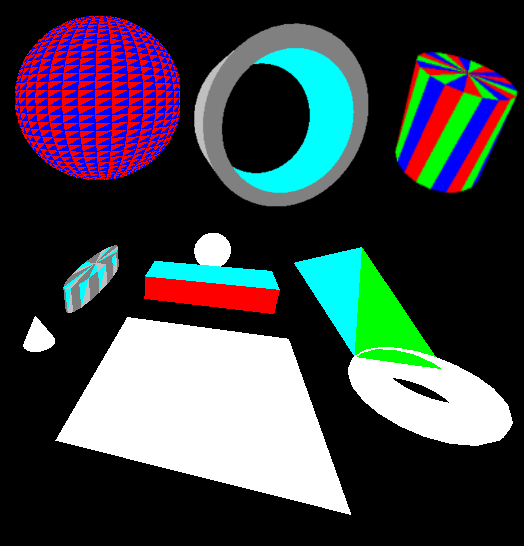
\includegraphics[width=0.9\textwidth]{images/GraphicAllMesh.png}
        \caption{Les meshs du jeu sous leur forme brute} 
    \end{minipage}%
    \hfill
    \begin{minipage}{0.45\textwidth}
        \centering
        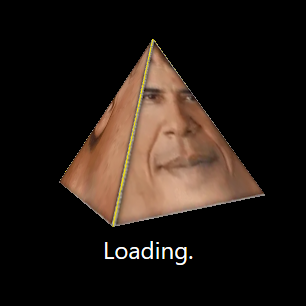
\includegraphics[width=0.9\textwidth]{images/GraphicLoadingScreen.png}
        \caption{Rendu du menu de chargement du jeu}
    \end{minipage}
    
    \vspace{1em} % Espacement vertical entre les lignes
    
    \begin{minipage}{0.45\textwidth}
        \centering
        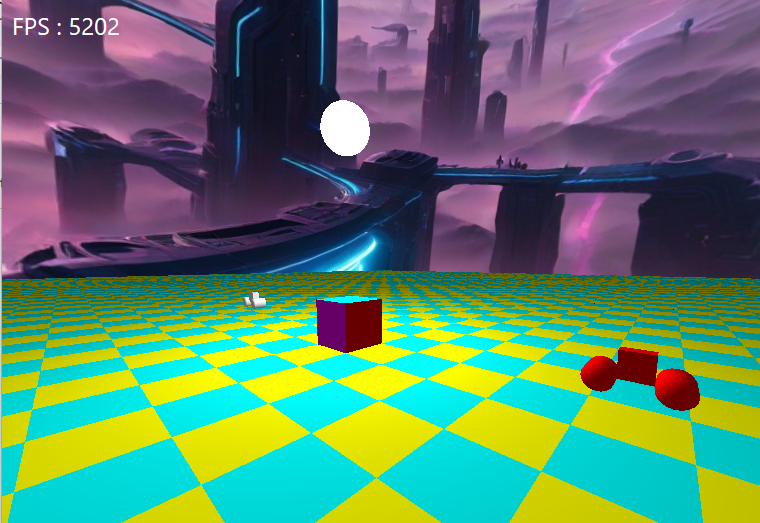
\includegraphics[width=\textwidth]{images/GraphicFirstGame.png}
        \caption{Premiers tests du jeu avec une grille et des joueurs}
    \end{minipage}%
    \hfill
    \begin{minipage}{0.45\textwidth}
        \centering
        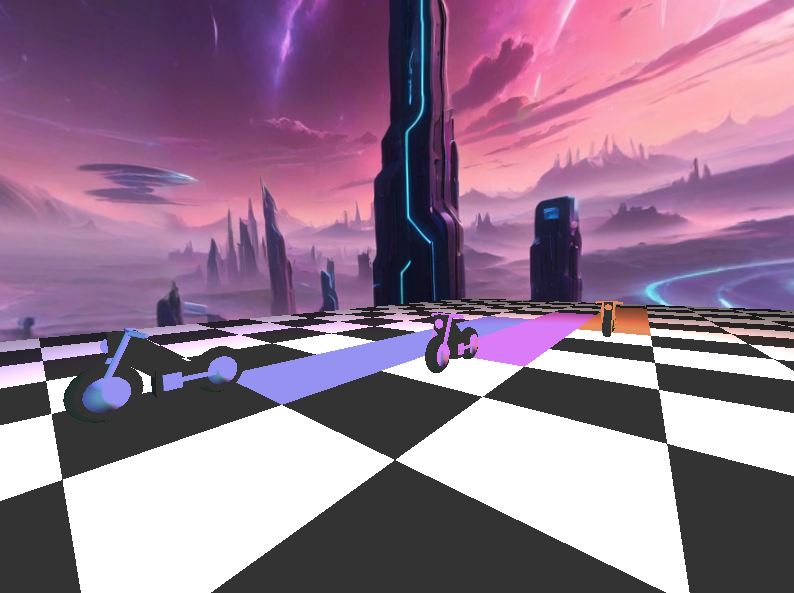
\includegraphics[width=0.9\textwidth]{images/GraphicFinalGame.png}
        \caption{Rendu final du jeu avec une grille et des joueurs}
    \end{minipage}
\end{figure}